\documentclass[9pt,academicons]{article}

\usepackage{CADA}
\usepackage{color}
\usepackage[table]{xcolor}
\definecolor{light-gray}{gray}{0.8}
\definecolor{light-light-gray}{gray}{0.9}

\title{Notes on the CAD-Compatible Conversion of Multi-Sided Surfaces}

\begin{document}


\maketitle

\authorSection{
	\anAuthor{P\'eter Salvi}{0000-0003-2456-2051}{1},
	\anAuthor{Tam\'as V\'arady}{0000-0001-9547-6498}{2},
	\anAuthor{Alyn Rockwood}{}{3}
}

\affiliationSection{
	\anAffiliation{1}{Budapest University of Technology and Economics}{salvi@iit.bme.hu}
	\anAffiliation{2}{Budapest University of Technology and Economics}{varady@iit.bme.hu}
	\anAffiliation{3}{Boulder Graphics LLC, USA}{alynrock@gmail.com}
}

\correspondingAuthor{P\'eter Salvi}{salvi@iit.bme.hu}

\abstract{
  Blah blah blah
}

\keywords{multi-sided surfaces, trimmed surfaces, S-patch, Charrot--Gregory patch} 

\doi{10.14733/cadaps.2021.aaa-bbb}

\section{INTRODUCTION}
\label{sec:intro}
Blah blah blah \cite{DeRose:1993} and \cite{Loop:1990} and \cite{Salvi:2019:KEPAF}
and \cite{Salvi:2019:WAIT}.

\section{INTERESTING DEVELOPMENTS}
\label{sec:interesting}

\begin{figure}
%\centering
\begin{subfigure}{.5\textwidth}
  \centering
  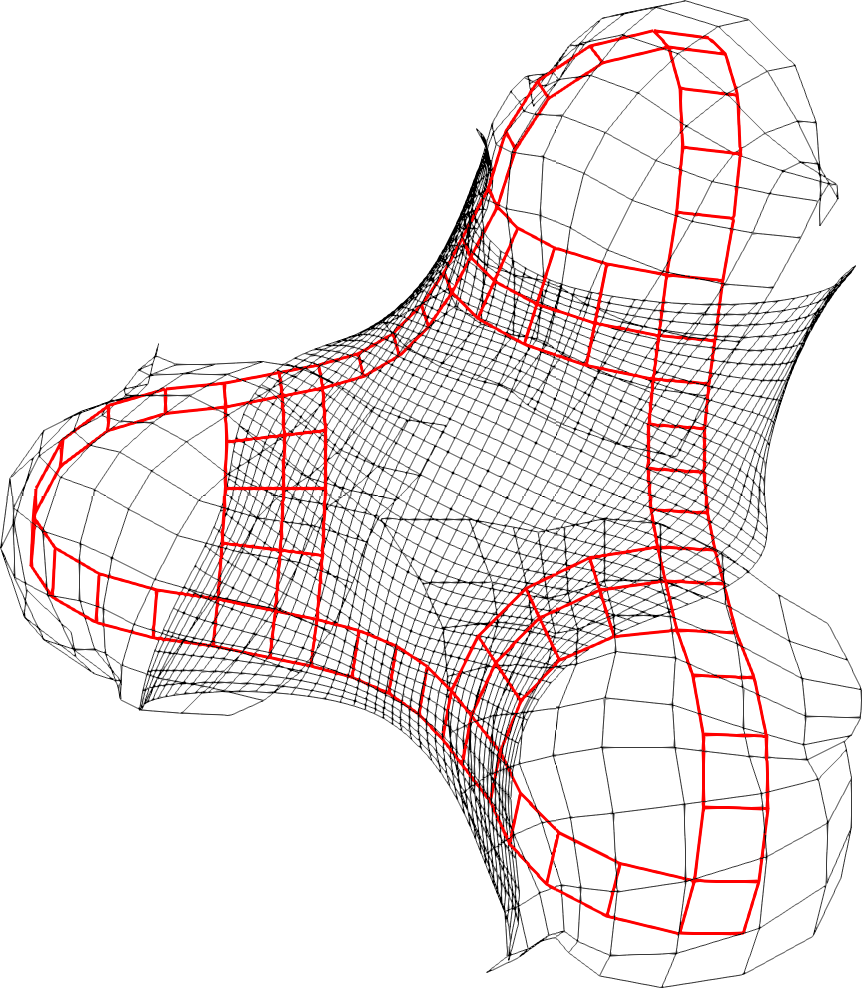
\includegraphics[height=.25\textheight]{images/trebol3-cnet.png}
  \caption{Many control points!}
\end{subfigure}
\begin{subfigure}{.5\textwidth}
  \centering
  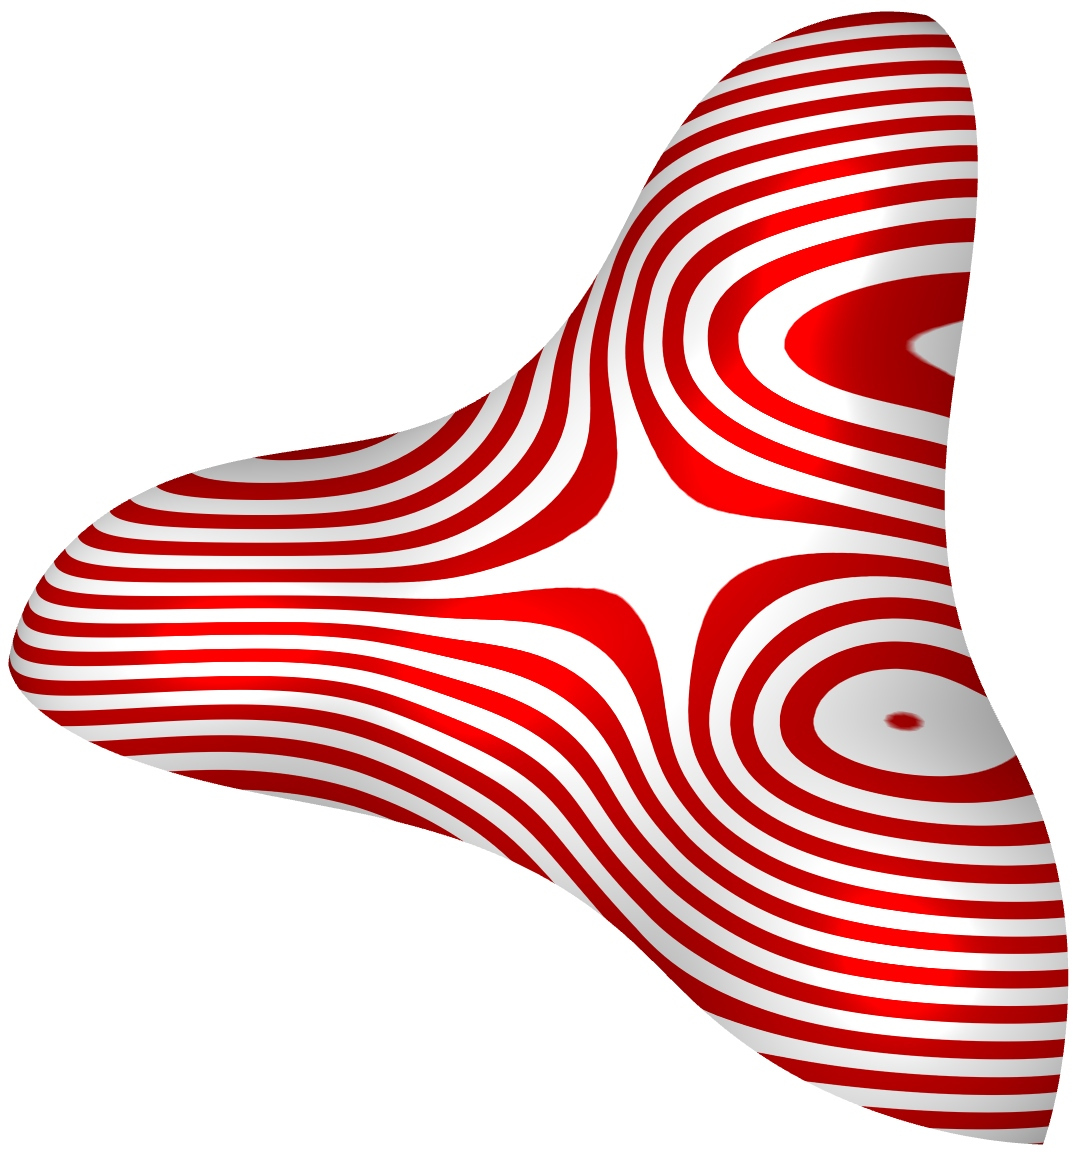
\includegraphics[height=.25\textheight]{images/trebol3-zebra.jpg}
  \caption{Nice isophotes!}
\end{subfigure}
\caption{Trebol model}
\label{fig:trebol}
\end{figure}

\begin{table}[h!]
  \centering
  \begin{tabular}{c|c|c|c|c}
    $n$ & S-patch~\cite{Loop:1989} & Warren~\cite{Warren:1992} & Kato~\cite{Kato:1991} & Charrot--Gregory~\cite{Charrot:1984} \\ \hline
    3 & \multicolumn{2}{c|}{$d[+3]$ (both B\'ezier triangles)} & \cellcolor{light-gray}$3d+5$ & $d+3$ \\ \hline
    5 & \cellcolor{light-light-gray}$3d[+9]$ & $\approx 3d$ & \cellcolor{light-gray}$5d+9$ & $5d+6$ \\ \hline
    6 & \cellcolor{light-light-gray}$4d[+12]$ & $3d$ & \cellcolor{light-gray}$6d+11$ & $6d+8$ \\ \hline
    7+ & \cellcolor{light-gray}$(n-2)(d[+3])$ & $\qquad$N/A$\qquad$ & \cellcolor{light-gray}$nd+2n-1$ & \cellcolor{light-gray}$nd+2n-4$ \\ \hline
  \end{tabular}
  \caption{Rational polynomial degrees of the converted surfaces for different number of sides,
    assuming boundary curves of degree $d$. Gray cells indicate that the surface is susceptible to
    the singularity issue.
    For S-patches, the number in brackets is applied
    when the surface is generated by a degree-$d$ $G^1$ frame.}
  \label{tab:degrees}
\end{table}

\subsection{Results}
Blah blah blah

\section{CONCLUSIONS}

Blah blah blah

\section*{ACKNOWLEDGEMENTS}
Blah blah blah

\section*{ORCID}
\orcid{P\'eter Salvi}{0000-0003-2456-2051}
\orcid{Tam\'as V\'arady}{0000-0001-9547-6498}

\referenceSection
\bibliographystyle{CADA}
\bibliography{cikkek}

\bigskip
\end{document}
